\documentclass[]{article}
\usepackage{lmodern}
\usepackage{amssymb,amsmath}
\usepackage{ifxetex,ifluatex}
\usepackage{fixltx2e} % provides \textsubscript
\ifnum 0\ifxetex 1\fi\ifluatex 1\fi=0 % if pdftex
  \usepackage[T1]{fontenc}
  \usepackage[utf8]{inputenc}
\else % if luatex or xelatex
  \ifxetex
    \usepackage{mathspec}
  \else
    \usepackage{fontspec}
  \fi
  \defaultfontfeatures{Ligatures=TeX,Scale=MatchLowercase}
\fi
% use upquote if available, for straight quotes in verbatim environments
\IfFileExists{upquote.sty}{\usepackage{upquote}}{}
% use microtype if available
\IfFileExists{microtype.sty}{%
\usepackage{microtype}
\UseMicrotypeSet[protrusion]{basicmath} % disable protrusion for tt fonts
}{}
\usepackage[margin=1in]{geometry}
\usepackage{hyperref}
\hypersetup{unicode=true,
            pdftitle={On the inference of positive and negative species interactions and their relation to abundance},
            pdfauthor={Andrew J. Rominger},
            pdfborder={0 0 0},
            breaklinks=true}
\urlstyle{same}  % don't use monospace font for urls
\usepackage{graphicx,grffile}
\makeatletter
\def\maxwidth{\ifdim\Gin@nat@width>\linewidth\linewidth\else\Gin@nat@width\fi}
\def\maxheight{\ifdim\Gin@nat@height>\textheight\textheight\else\Gin@nat@height\fi}
\makeatother
% Scale images if necessary, so that they will not overflow the page
% margins by default, and it is still possible to overwrite the defaults
% using explicit options in \includegraphics[width, height, ...]{}
\setkeys{Gin}{width=\maxwidth,height=\maxheight,keepaspectratio}
\IfFileExists{parskip.sty}{%
\usepackage{parskip}
}{% else
\setlength{\parindent}{0pt}
\setlength{\parskip}{6pt plus 2pt minus 1pt}
}
\setlength{\emergencystretch}{3em}  % prevent overfull lines
\providecommand{\tightlist}{%
  \setlength{\itemsep}{0pt}\setlength{\parskip}{0pt}}
\setcounter{secnumdepth}{0}
% Redefines (sub)paragraphs to behave more like sections
\ifx\paragraph\undefined\else
\let\oldparagraph\paragraph
\renewcommand{\paragraph}[1]{\oldparagraph{#1}\mbox{}}
\fi
\ifx\subparagraph\undefined\else
\let\oldsubparagraph\subparagraph
\renewcommand{\subparagraph}[1]{\oldsubparagraph{#1}\mbox{}}
\fi

%%% Use protect on footnotes to avoid problems with footnotes in titles
\let\rmarkdownfootnote\footnote%
\def\footnote{\protect\rmarkdownfootnote}

%%% Change title format to be more compact
\usepackage{titling}

% Create subtitle command for use in maketitle
\newcommand{\subtitle}[1]{
  \posttitle{
    \begin{center}\large#1\end{center}
    }
}

\setlength{\droptitle}{-2em}

  \title{On the inference of positive and negative species interactions and their
relation to abundance}
    \pretitle{\vspace{\droptitle}\centering\huge}
  \posttitle{\par}
    \author{Andrew J. Rominger}
    \preauthor{\centering\large\emph}
  \postauthor{\par}
    \date{}
    \predate{}\postdate{}
  
\usepackage{xr}
\externaldocument{RarePlusComMinus_supp}

\begin{document}
\maketitle

Why do rare species persist in ecosystems? Rare species seem to be at a
disadvantage by pure probabilistic odds\textsuperscript{1} and perhaps
also from poorly adapted species-environment and species-species
interactions\textsuperscript{2}, though negative density-dependence may
help rare species persist\textsuperscript{3,4}. The question of rarity
and persistence thus remains unresolved. In a recent paper, Calatayuda
et al.\textsuperscript{5} (CEA) have contributed toward helping resolve
this question. They compiled an impressive collection of datasets,
across many taxa and environments, capturing spatially replicated
species abundance measures. With these data they inferred
species-species interaction networks. CEA found that rare species were
statistically associated with positive interactions whereas common
species were associated with negative interactions, indicating that
positive interactions, such as facilitation, may help rare species
persist\textsuperscript{5}. However, the use of abundance data to infer
species interactions is difficult and often
inaccurate\textsuperscript{6--8}. Here, I show that the finding of an
association between abundance and interaction type as reported by CEA
can be explained by statistical artifacts in the inference of species
interactions from abundance data. These artifacts arise because of
spatial clustering in species abundances. It would therefore not be
supported to assign biological interpretations to associations between
interaction types and abundances until more data can be brought to bear
on the subject of interaction types and the persistence of rare species.

When interaction networks are inferred from spatially replicated
abundance data, species-species co-occurrences are quantified by a
metric (e.g., CEA use Schoener similarity\textsuperscript{9}) and then a
null model is used to assess whether these co-occurrence metrics deviate
substantially enough from null expectations to suggest a non-random
interaction, either in the positive direction (suggesting positive
interactions) or the negative direction (suggesting negative
interactions). However, if abundances are driven by processes, both
probabilistic or deterministic, other than species-species interactions,
these null models may not reveal true interactions, but rather artifacts
of other processes. Species abundances are not evenly distributed within
species nor across space (often referred to as spatial
clustering)\textsuperscript{10--14}. This ubiquitous pattern can be
accounted for by purely probabilistic processes from neutral
birth-death-immigration\textsuperscript{15} to mechanistically agnostic
statistical-mechanical properties of large
assemblages\textsuperscript{13}. Thus, the simple observation of uneven
abundances does by itself indicate the influence of deterministic
species interactions. The data compiled by CEA\textsuperscript{5} indeed
confirm the ubiquity of uneven species abundances (Supplementary Figs.
\ref{fig:ssad} and \ref{fig:sadShape}).

In Figure \ref{fig:plusMinus} I first reproduce key results from CEA's
Figure 2(B-C). Then to evaluate whether these results can be produced
simply from spatial clustering alone I simulate purely random data that
match the unevenness of abundance found in the observed data but contain
absolutely no species interactions. These random data are simulated as
follows:

\begin{enumerate}
\def\labelenumi{\arabic{enumi})}
\tightlist
\item
  The number of species \(S\), number of sites \(M\), and shape of the
  best fitting species abundance distribution (SAD) are sampled (with
  replacement) from the observed data
\item
  \(S\) species abundances \(x_i \ldots x_S\) are sampled from the SAD
\item
  For each \(x_i\), within-species counts are distributed across the
  \(M\) sites according to a spatial species abundance distribution
  (SSAD) that is either negative binomial (in the case of spatial
  clustering) or Poisson (in the case of spatial evenness)
\item
  The resulting simulated site by species matrix is fed through the same
  analytically pipeline (described in CEA) as the observed data to infer
  positive and negative interactions.
\end{enumerate}

All analyses are carried out in R\textsuperscript{17} and can be fully
reproduced by installing the R package accompanying this paper, as
detailed in the supplement.

\begin{figure}

{\centering 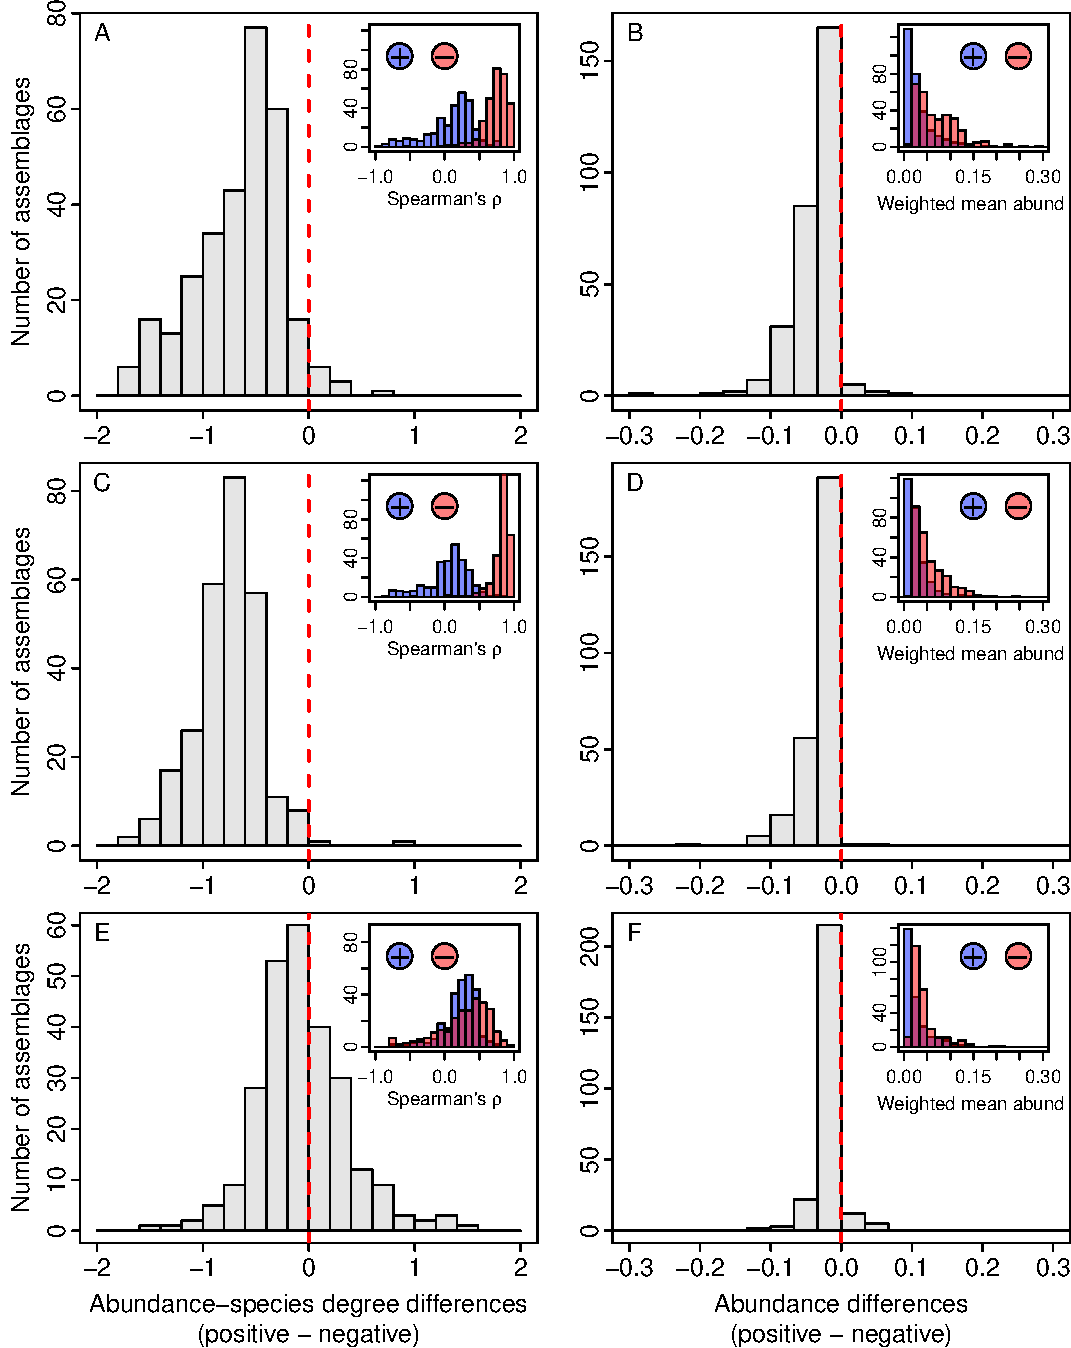
\includegraphics{RarePlusComMinus_files/figure-latex/fig_plusMinus-1} 

}

\caption{Distributions of correlations between network centrality (i.e. species degree) and abundance (left panels) and distributions of weighted mean abundances (right panels). The main figures show the differences between positive and negative interaction networks, while the inset figures show the sepparate distributions for each network. The results of CEA Figure 2(B-C) are reproduced here in panels A-B; panels C-D show data simulated with a negative binomial SSAD and no species interactions; panels E-F show data simulated with a Poisson SSAD and no species interactions. \label{fig:plusMinus}}\label{fig:fig_plusMinus}
\end{figure}

In the case of a Poisson SSAD the one parameter (the mean) is fully
specified by the average site-level abundance of a given species. In the
case of a negative binomial SSAD, the mean parameter is again specified
by the site-level average, but the size or clustering parameter \(k\) is
not fully specified. To capture the rough features of the data, I sample
\(k\) from a linear relationship (with noise) between the maximum
likelihood estimates of \(k\) and the relative abundance of each species
(Supplementary Fig. \ref{fig:ssad}).

Figure \ref{fig:plusMinus} A--D shows that with a negative binomial
SSAD, simulated data closely match observed findings: the correlation
between abundance and species' network degree skews more negative in
positive interaction networks (i.e.~more rare species are more highly
connected in positive interaction networks), and positive interaction
networks tend to contain more rare species than negative networks. This
correspondence between real and simulated patterns largely disappears
when we instead use a Poisson SSAD, highlighting the importance of
spatial aggregation in driving the spurious results.

My findings do not depend on simulating SAD and SSAD shapes from the
data: in Supplementary Figure \ref{fig:simpleSim} I show that the
spurious relationship between abundance and interaction type occurs even
when simulating data from just one arbitrary SAD function with the one
arbitrary spatially clustered SSAD for all species. In this simulation,
again, replacing the spatially clustered SSAD with a Poisson SSAD breaks
the spurious association as in Figure \ref{fig:plusMinus} (E-F).

Why do negative binomial SSADs reproduce the results while Poisson SSADs
fail to? The null model algorithm used here and in CEA fixes row and
column marginals, but within any given species, the way its total
abundance is allocated across sites by the null model has a potentially
large combinatorial space to explore. I compare known SSADs to their
permuted counterpart in Figure \ref{fig:ssadPerm} and find that the null
model transforms negative binomial SSADs to a more Poisson shape, while
leaving Poisson SSADs probabilistically unchanged. Specifically, when
starting with a negative binomial SSAD, the null model inflates the
number of sites individuals are allocated to (more similarly to a
Poisson SSAD) and increases the inferred \(k\) parameter, indicating
less spatial clustering in the permuted matrices compared to their
non-permuted, negative binomial starting points.

\begin{figure}

{\centering 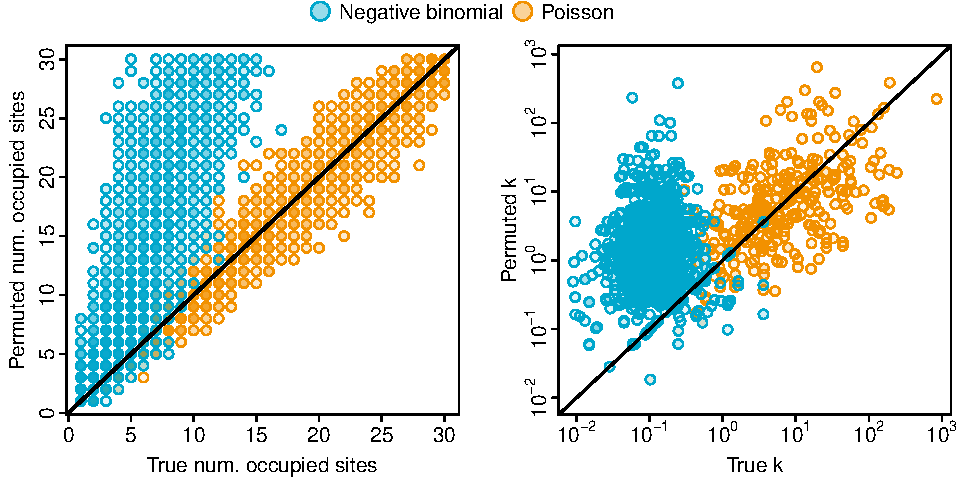
\includegraphics{RarePlusComMinus_files/figure-latex/ssadPerm_plot-1} 

}

\caption{Comparison of SSAD statistics for true and permuted site by species matrices. Colors correspond to the true, un-permuted SSAD. Panel (A) shows how permutation affects number of occupied sites. Panel (B) shows how permutation affects maximum likelihood estimates of the clustering parameter $k$ (B). Points are semi-transparent to help display density. Lines are 1:1 lines. \label{fig:ssadPerm}}\label{fig:ssadPerm_plot}
\end{figure}

At a mathematical level, clustered SSADs, compared to spatially even
SSADs, actually increase the probability that rare species will appear
aggregated with each other and common species will appear repelled.
Consider for example two rare species, one with a single individual and
the other with abundance 5, distributed across 5 sites. Their Schoener
similarity is maximized when all individuals occur at the same site,
such as this site by species matrix \[
X_{rare} = \begin{bmatrix} 1 & 5 \\ 0 & 0 \\ 0 & 0 \\ 0 & 0 \\ 0 & 0 \\ \end{bmatrix}
\] If we define \(Q(x_i; \mu = 1)\) as the probability of observing
\(x_i\) individuals in site \(i\) given an SSAD with mean parameter
\(\mu\), then the probability of the above configuration is
\(P(X_{rare}) = Q(5; \mu = 1) \left(Q(0; \mu = 1)^{4}\right)\). Under a
negative binomial SSAD with \(k = 0.1\),
\(P(X_{rare}) = 4.58 \times 10^{-3}\) whereas under a Poisson SSAD
\(P(X_{rare}) = 5.61 \times 10^{-5}\).

Conversely, for two common species, say each with abundance 50, an
example configuration that \emph{minimizes} their Schoener similarity
would be \[
Y_{min} = \begin{bmatrix} 50 & 0 \\ 0 & 50 \\ 0 & 0 \\ 0 & 0 \\ 0 & 0 \\ \end{bmatrix}
\] We calculate the probability of any such scenario where no abundances
overlap as
\(P(Y_{min}) = 4 \left(\left(Q(50; \mu = 10) Q(0; \mu = 10)^{4}\right)^2\right)\).
With a negative binomial SSAD with \(k = 0.1\),
\(P(Y_{min}) = 1.41 \times 10^{-7}\) whereas with a Poisson SSAD
\(P(Y_{min}) = 1.61 \times 10^{-72}\).

We contrast this with a configuration that would maximize the Schoener
similarity between these two common species: \[
Y_{max} = \begin{bmatrix} 10 & 10 \\ 10 & 10 \\ 10 & 10 \\ 10 & 10 \\ 10 & 10 \\ \end{bmatrix}
\] The probability of this configuration is
\(P(Y_{max}) = Q(10; \mu = 10)^{10}\). For the same negative binomial
\(P(Y_{max}) = 5.76 \times 10^{-22}\), and for the Poisson
\(P(Y_{max}) = 9.40 \times 10^{-10}\).

Thus a spatially clustered SSAD, compared to a spatially even SSAD,
gives more probability to configurations where rare species appear
aggregated and common species appear over-dispersed. Because the null
model algorithm permutes site by species matrices to resemble more
spatially even SSADs this probabilistic difference between spatially
clustered versus even SSADs accounts for the prevalence of rare species
in positive interaction networks and common species in negative
interaction networks.

Great caution should be used when inferring species interactions from
abundance data. More fundamentally than the spurious association of
abundance with interaction type, my analysis shows that statistically
significant species interactions are inferred from data simulated
without any interactions. In data simulated with a negative binomial
SSAD, on average 75\% of species were placed in positive interaction
networks and 74\% in negative interaction networks with a significance
cutoff of \(\alpha = 0.05\). With the Poisson SSAD these simulated
numbers were 71\% for positive networks and 25\% for negative networks.
For the observed data, on average 73\% of species were placed in
positive interaction networks and 60\% in negative interaction networks.
It is becoming increasingly appreciated that abundance data alone are
not sufficient to distinguish between different ecological
processes\textsuperscript{18,19}. The question of why rare species
persist is fascinating, and CEA should be commended for making a
concerted effort to illuminate possible mechanisms underlying the
phenomenon; however, to reach robust conclusions, other types of data,
such as actual experimental measurement of interaction strengths, are
needed in addition to abundance data.

\clearpage

\section*{References}\label{references}
\addcontentsline{toc}{section}{References}

\hypertarget{refs}{}
\hypertarget{ref-mcgill2005}{}
1. McGill, B. J., Hadly, E. A. \& Maurer, B. A. Community inertia of
quaternary small mammal assemblages in north america. \emph{Proceedings
of the National Academy of Sciences} \textbf{102}, 16701--16706 (2005).

\hypertarget{ref-hutchinson1961}{}
2. Hutchinson, G. E. The paradox of the plankton. \emph{The American
Naturalist} \textbf{95}, 137--145 (1961).

\hypertarget{ref-leigh2004}{}
3. Leigh Jr, E. G. \emph{et al.} Why do some tropical forests have so
many species of trees? \emph{Biotropica} \textbf{36}, 447--473 (2004).

\hypertarget{ref-yenni2012}{}
4. Yenni, G., Adler, P. B. \& Ernest, S. M. Strong self-limitation
promotes the persistence of rare species. \emph{Ecology} \textbf{93},
456--461 (2012).

\hypertarget{ref-calatayud2019}{}
5. Calatayud, J. \emph{et al.} Positive associations among rare species
and their persistence in ecological assemblages. \emph{Nat Ecol Evol}
(2019).

\hypertarget{ref-freilich2018}{}
6. Freilich, M. A., Wieters, E., Broitman, B. R., Marquet, P. A. \&
Navarrete, S. A. Species co-occurrence networks: Can they reveal trophic
and non-trophic interactions in ecological communities? \emph{Ecology}
\textbf{99}, 690--699 (2018).

\hypertarget{ref-carr2019}{}
7. Carr, A., Diener, C., Baliga, N. S. \& Gibbons, S. M. Use and abuse
of correlation analyses in microbial ecology. \emph{The ISME journal}
\textbf{13}, 2647--2655 (2019).

\hypertarget{ref-rajala2019}{}
8. Rajala, T., Olhede, S. C. \& Murrell, D. J. When do we have the power
to detect biological interactions in spatial point patterns?
\emph{Journal of Ecology} \textbf{107}, 711--721 (2019).

\hypertarget{ref-schoener1968}{}
9. Schoener, T. W. The anolis lizards of bimini: Resource partitioning
in a complex fauna. \emph{Ecology} \textbf{49}, 704--726 (1968).

\hypertarget{ref-mcgill2003}{}
10. McGill, B. \& Collins, C. A unified theory for macroecology based on
spatial patterns of abundance. \emph{Evolutionary Ecology Research}
\textbf{5}, 469--492 (2003).

\hypertarget{ref-engen2008}{}
11. Engen, S., Lande, R. \& Sæther, B.-E. A general model for analyzing
taylor's spatial scaling laws. \emph{Ecology} \textbf{89}, 2612--2622
(2008).

\hypertarget{ref-zillio2010}{}
12. Zillio, T. \& He, F. Modeling spatial aggregation of finite
populations. \emph{Ecology} \textbf{91}, 3698--3706 (2010).

\hypertarget{ref-harte2011}{}
13. Harte, J. \emph{The maximum entropy theory of ecology}. (Oxford
University Press, 2011).

\hypertarget{ref-connolly2017}{}
14. Connolly, S. R., Hughes, T. P. \& Bellwood, D. R. A unified model
explains commonness and rarity on coral reefs. \emph{Ecology letters}
\textbf{20}, 477--486 (2017).

\hypertarget{ref-kendall1949}{}
15. Kendall, D. G. Stochastic processes and population growth.
\emph{Journal of the Royal Statistical Society. Series B
(Methodological)} \textbf{11}, 230--282 (1949).

\hypertarget{ref-hubbell2001}{}
16. Hubbell, S. P. \emph{The unified neutral theory of biodiversity and
biogeography}. (Princeton University Press, 2001).

\hypertarget{ref-rcore}{}
17. R Core Team. \emph{R: A language and environment for statistical
computing}. (R Foundation for Statistical Computing, 2018).

\hypertarget{ref-mcgill2007}{}
18. McGill, B. J. \emph{et al.} Species abundance distributions: Moving
beyond single prediction theories to integration within an ecological
framework. \emph{Ecology letters} \textbf{10}, 995--1015 (2007).

\hypertarget{ref-morlon2009}{}
19. Morlon, H. \emph{et al.} Taking species abundance distributions
beyond individuals. \emph{Ecology Letters} \textbf{12}, 488--501 (2009).


\end{document}
